\chapter{Train Benchmark Implementation}

In this chapter, we discuss the implementation details of the Train Benchmark. The installation guide is available in the MONDO wiki.\footnote{\url{https://opensourceprojects.eu/p/mondo/wiki/TrainBenchmark/}}

\section{Performance Benchmark Framework}

\subsection{Architecture}

For the integration of the Train Benchmark projects and their third party dependencies, we use Apache Maven~\cite{Maven}. The dependencies are shown in \figref{fig:trainbenchmark-modules}.

\begin{figure}[!Htb]
	\centering
	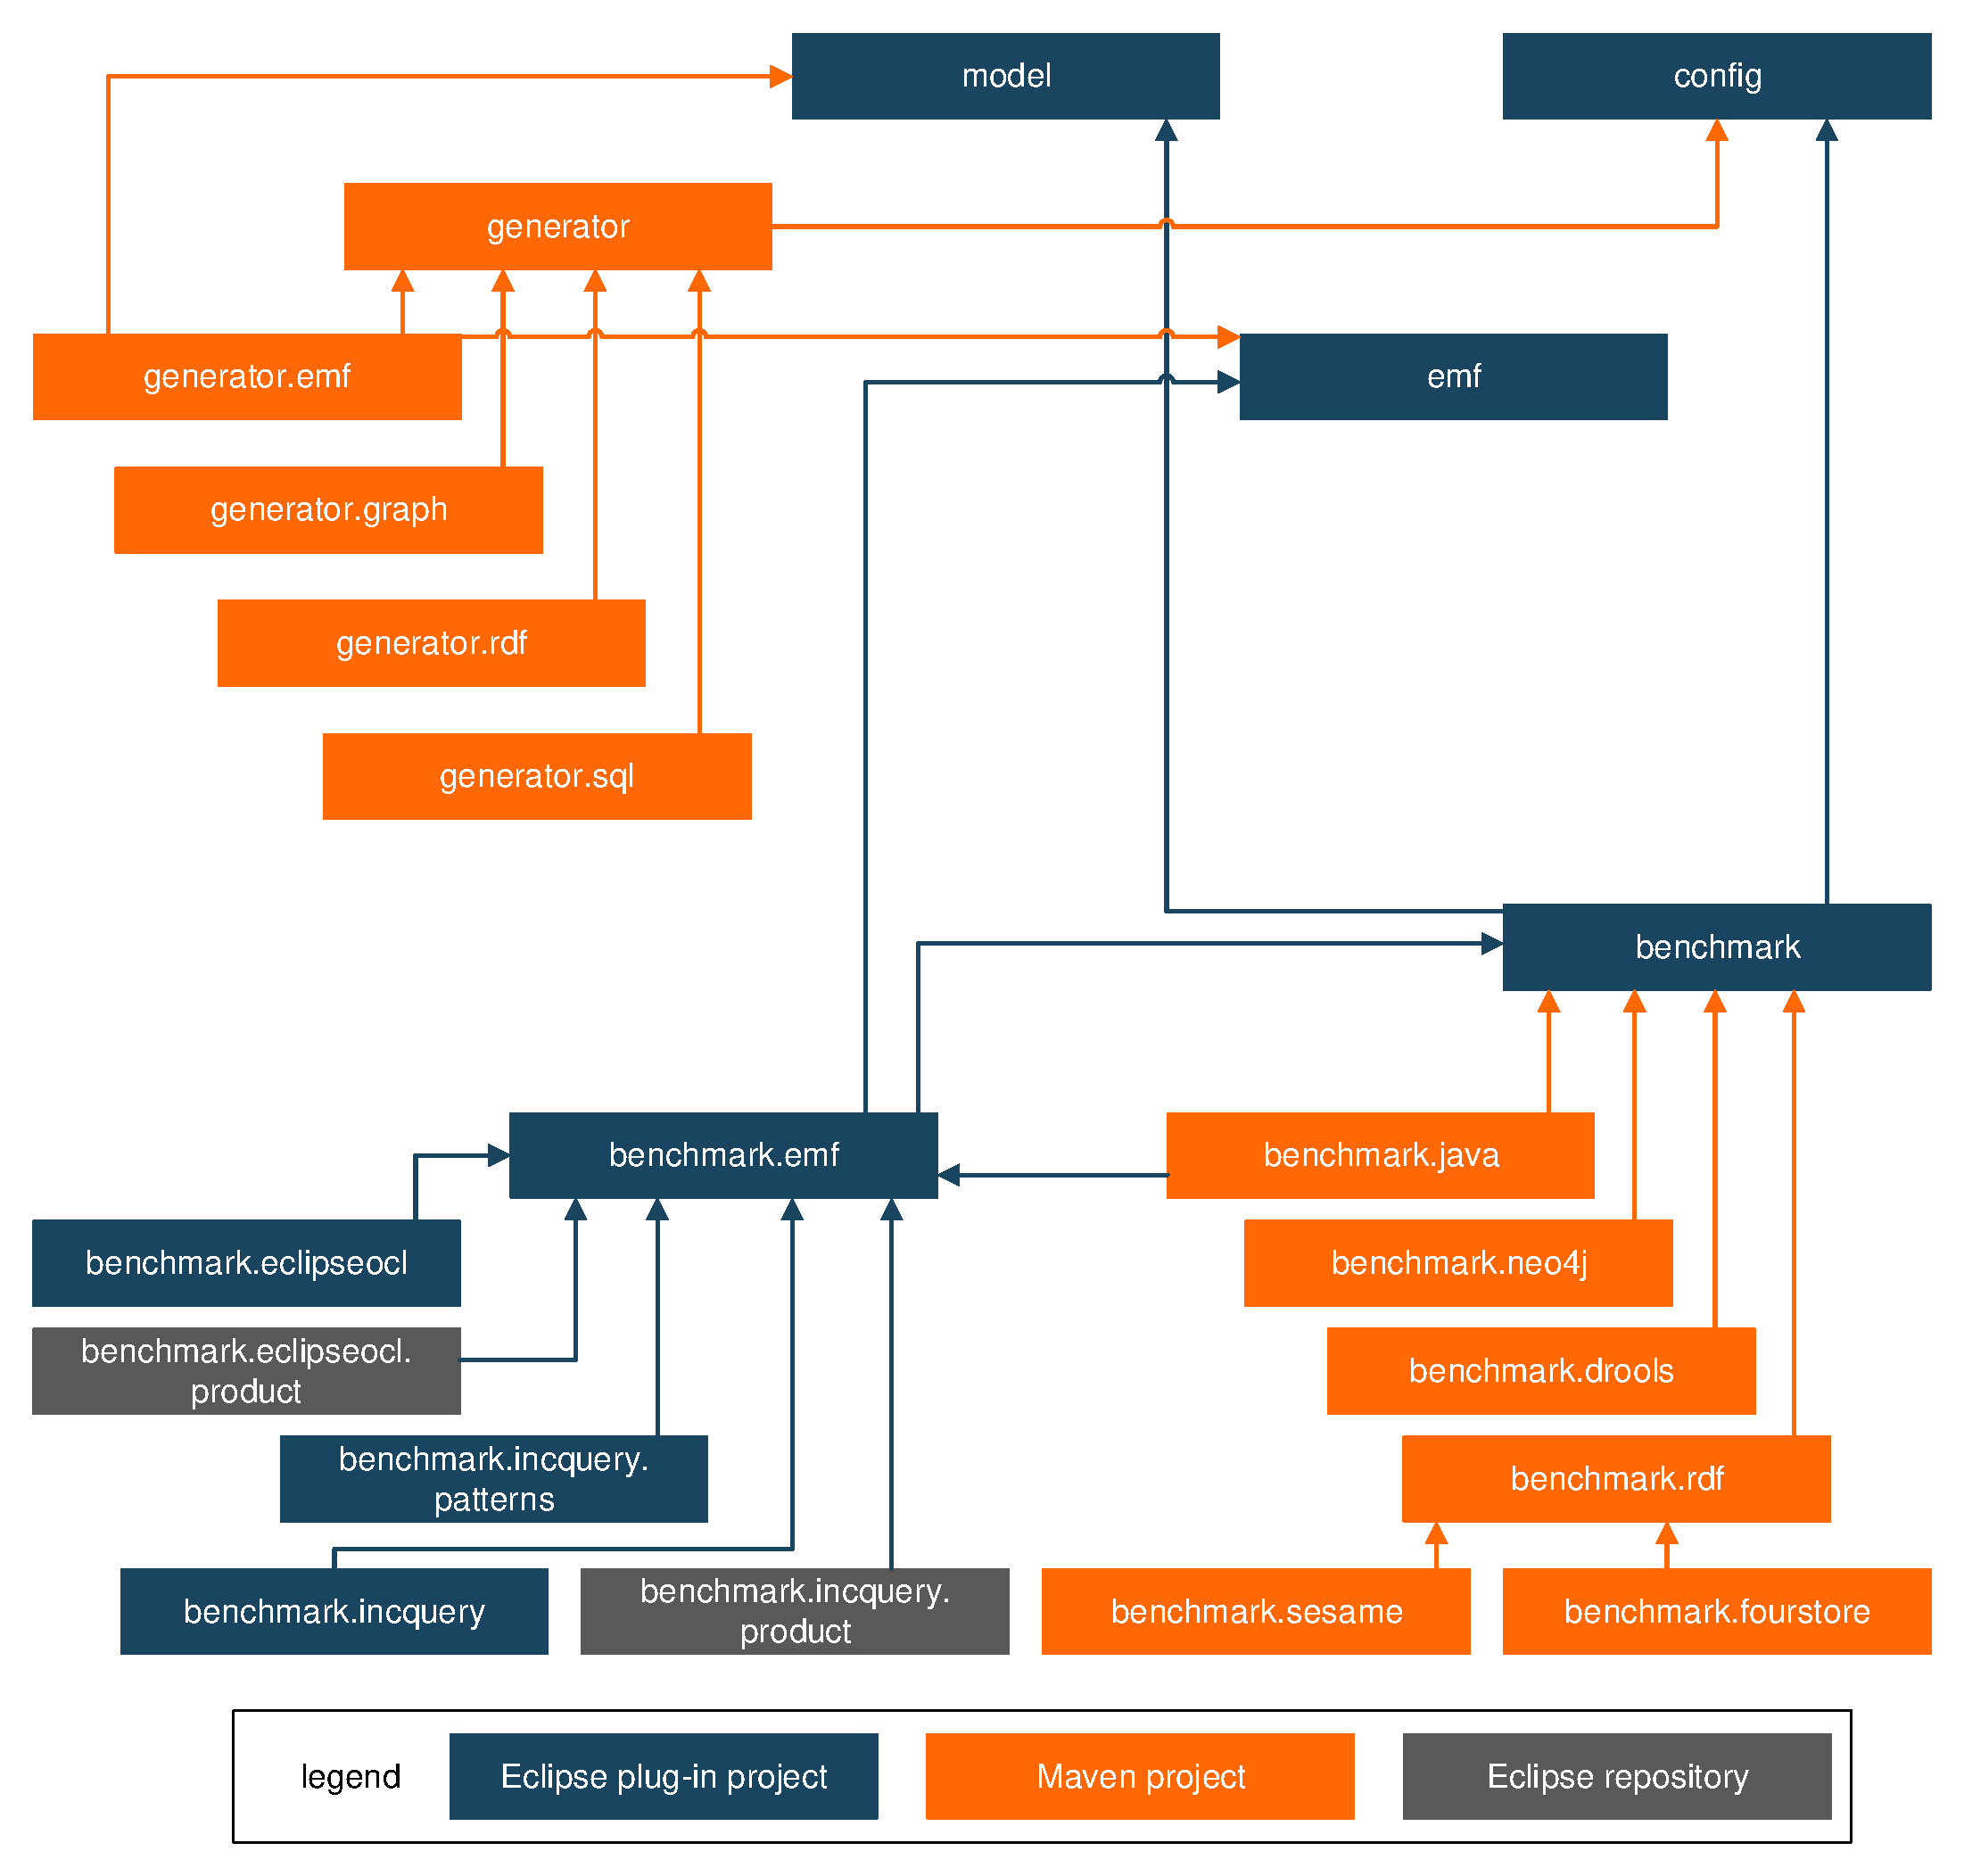
\includegraphics[width=\textwidth]{figures/trainbenchmark-modules}
	\caption{The Maven modules defined in the Train Benchmark. Note that artifact ids of the modules are shortened and the full ids start with \texttt{hu.bme.mit.trainbenchmark}.}
	\label{fig:trainbenchmark-modules}
\end{figure}

In this section, we briefly describe the tasks and responsibilities of each module.

\subsubsection{Parent module}

The \texttt{hu.bme.mit.trainbenchmark} module is the parent module which contains the modules used in the Train Benchmark. Building this Maven module builds all child modules as well.

\subsubsection{Central modules}

The \texttt{hu.bme.mit.trainbenchmark.model} module contains the reference metamodel represented in EMF.

The \texttt{hu.bme.mit.trainbenchmark.config} module contains classes and constants used by the \texttt{generator} and the \texttt{benchmark} projects.

\subsubsection{Representation-specific modules}

The \texttt{hu.bme.mit.trainbenchmark.emf} and \texttt{hu.bme.mit.trainbenchmark.rdf} modules contain classes and constants used by the particular representations.

\subsubsection{Generator modules}

The \texttt{hu.bme.mit.trainbenchmark.generator.*} modules are responsible for generating the instance models for the benchmarks.

\begin{itemize}
  \item \texttt{emf}: generates an EMF instance model.
  \item \texttt{graph}: generates a property graph model in the specified format: GraphML (default), Blueprints GraphSON, Faunus GraphSON.
  \item \texttt{rdf}: generates an RDF instance model.
  \item \texttt{sql}: generates an SQL script which creates and loads the appropriate database tables.
\end{itemize}


\subsubsection{Benchmark modules}

The \texttt{hu.bme.mit.trainbenchmark.benchmark.*} modules are responsible for benchmarking. For the list of current implementations, see \autoref{tbl:tools}.

\subsubsection{4store}

To access 4store through a graph-like API, we developed a Java client\footnote{\url{https://git.inf.mit.bme.hu/w?p=projects/bigmodel/4store-graph-client.git}, \\ clone URI: \url{git@git.inf.mit.bme.hu:projects/bigmodel/4store-graph-client.git}} with a focus on high performance.

%\subsection{Extending the framework with custom tools, queries or models}
%\subsubsection{Extending the model generator with new syntaxes}
%\subsubsection{Adding a tool to measure performance}

\subsection{Generating diagrams automatically}

\subsubsection{Dependencies}

\begin{enumerate}
  \item Go to the \texttt{src/hu.bme.mit.trainbenchmark.analyze} in the \texttt{mondo-trainbenchmark} repository.
  \item Install R, install the \texttt{r-base}, \texttt{r-base-dev} package.
  \item If you wish to edit the R files, it is strongly recommended to install RStudio.\footnote{\url{http://www.rstudio.com/ide/download/desktop}}.
  \item Install the required R packages by issuing the following command: \texttt{R --file=install.R}. 
\end{enumerate}

\subsubsection{Steps to generate diagrams automatically}

\begin{enumerate}
  \item Go to the \texttt{src/hu.bme.mit.trainbenchmark.analyze} in the \texttt{mondo-trainbenchmark} repository.
  \item Merge the measured data into \texttt{results.txt}. The file contains one header line and multiple data records belonging to (optionally) multiple series.
  \item Modify \texttt{configs.R} to introduce a new tool (specify the name of the tool in the \texttt{results.txt} file and on the diagrams), specify the line color and the type of the tool and in the \texttt{drawtools} variable enumerate tools to be plotted.
  \item Execute the \texttt{knitIt.sh} script.
  \item Inspect the generated \texttt{plotLines.html} and \texttt{plotLines-user.html} reports.
  \item If the you want the report to be zipped in a single file, execute \texttt{packHTML.sh} that generates \texttt{tbReport.zip}.
\end{enumerate}

\subsection{Command-line arguments}

All runnable Train Benchmark projects are configured through command-line arguments:

\begin{lstlisting}[keywordstyle=\ttfamily]
 -scenario <arg>               Batch/User/XForm
 -sizes <arg>                  model sizes, e.g. 4 or 1-8 or 1,8-512
 -workspacePath <arg>          path of the Eclipse workspace with all projects
\end{lstlisting}

The \texttt{benchmark} projects have additional arguments:

\begin{lstlisting}[keywordstyle=\ttfamily]
 -benchmarkMode <arg>                                      run benchmark specific (non-functional) procedures,
                                                                  like cleaning the OS cache
 -iterationCount <arg>                                     number of modify-check iterations
 -modificationConstant <arg>                               modification constant for the modification method
 -modificationConstantPosLength <arg>                      amount of modification for the PosLength test
 -modificationConstantRouteSensor <arg>                    amount of modification for the RouteSensor test
 -modificationConstantSignalNeighbor <arg>                 amount of modification for the SignalNeighbor test
 -modificationConstantSwitchSensor <arg>                   amount of modification for the SwitchSensor test
 -modificationMethod <arg>                                 options:
                                                           constant -- modify a fixed number of elements,
                                                           resultSet -- modify based a number of elements based on the size of the results set
 -queries <arg>                                            a comma-separated list of the queries to run,
                                                                  e.g. PosLength,RouteSensor
 -seriesCount <arg>                                        number of the run benchmark series
\end{lstlisting}

\subsection{Opening EMF install models}

If you would like to view the EMF instance models, right click the \texttt{hu.bme.mit.trainbenchmark.model} project and choose \textbf{Run As} | \textbf{Eclipse Application}) to start a new runtime Eclipse. Import the \texttt{hu.bme.mit.trainbenchmark.instancemodels} project. The \texttt{concept} files can be opened with the \textbf{Sample Reflective Model Editor}. (Warning: opening large models may cause the Eclipse instance to hang for a long time.)